\documentclass[../../../../main.tex]{subfiles}
\begin{document}

右の図において $ABC$ は長さ2の線分 $AB$ を直径とし，$O$ を中心とする半円周，
$P$ は $AB$ に垂直な半径 $OC$ 上の動点とする．

$k$ を正の定数とし，線分 $PO$ を $k:1$ に内分する点 $Q$ を通って $AB$ に平行な弦を $RS$ とすれば，
$P$ をどこにとったとき四辺形 $ROSP$ の面積が最大になるか．

\begin{figure}[htbp]
  \centering
  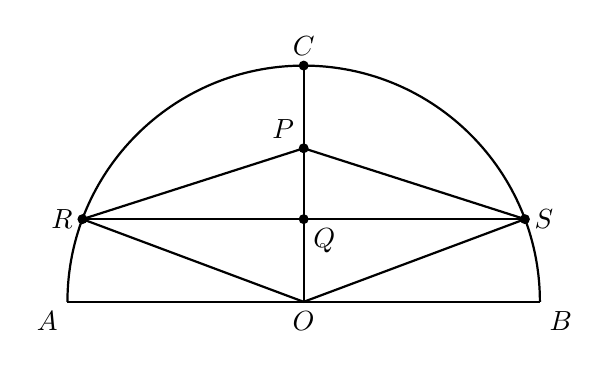
\begin{tikzpicture}[scale=1.5, >=stealth]
    \coordinate (A) at (-2,0);
    \coordinate (B) at (2,0);
    \coordinate (O) at (0,0);
    \coordinate (C) at (0,2);

    \draw[thick] (A) -- (B);
    \draw[thick] (2,0) arc (0:180:2);

    \draw[thick] (O) -- (C);

    \coordinate (P) at (0, 1.3);
    \coordinate (Q) at (0, 0.7);

    \coordinate (R) at (-1.873, 0.7);
    \coordinate (S) at (1.873, 0.7);

    \draw[thick] (R) -- (S);
    \draw[thick] (R) -- (O) -- (S) -- (P) -- cycle;

    \fill (P) circle (1.2pt) node[above left] {$P$};
    \fill (Q) circle (1.2pt) node[below right] {$Q$};
    \fill (R) circle (1.2pt) node[left] {$R$};
    \fill (S) circle (1.2pt) node[right] {$S$};
    \fill (C) circle (1.2pt) node[above] {$C$};

    \node[below left] at (A) {$A$};
    \node[below right] at (B) {$B$};
    \node[below] at (O) {$O$};
  \end{tikzpicture}
\end{figure}

\end{document}
